\documentclass[aspectratio=169,10pt]{beamer}
\usepackage[T1]{fontenc}
\usepackage[utf8]{inputenc}
\usepackage[brazil]{babel}
\usepackage{lmodern}
\usepackage{graphicx}
\usetheme{Boadilla}
\usefonttheme{professionalfonts}
\definecolor{AcademicBlue}{RGB}{27,52,82}
\definecolor{AcademicGray}{RGB}{88,97,107}
\setbeamercolor{structure}{fg=AcademicBlue}
\setbeamercolor{title}{fg=AcademicBlue}
\setbeamercolor{frametitle}{fg=AcademicBlue,bg=white}
\setbeamercolor{framesubtitle}{fg=AcademicGray}
\setbeamercolor{palette primary}{fg=AcademicBlue,bg=AcademicBlue!7}
\setbeamercolor{palette secondary}{fg=white,bg=AcademicBlue!85}
\setbeamercolor{palette tertiary}{fg=white,bg=AcademicBlue}
\setbeamertemplate{navigation symbols}{}
\setbeamertemplate{itemize items}[circle]
\setbeamertemplate{title page}[default][left]
\setbeamerfont{title}{size=\LARGE,series=\bfseries}
\setbeamerfont{subtitle}{size=\large}
\setbeamerfont{frametitle}{size=\Large,series=\bfseries}
\setbeamersize{text margin left=10mm,text margin right=10mm}
\title[ML Meets Networks]{Machine Learning Meets Networks}
\subtitle{Um guia prático para aplicações de aprendizado de máquina em redes sem fio e IoT}
\author[Donatti \& Fagundes]{Lorenzo Moreira Donatti\\Deivis Felipe Guerreiro Fagundes}
\institute[ERRC 2026]{Escola Regional de Redes de Computadores\\Minicurso intermediário\;\textperiodcentered\;150 minutos}
\date{2026}
\hypersetup{pdftitle={Machine Learning Meets Networks — ERRC 2026},pdfauthor={Lorenzo Moreira Donatti; Deivis Felipe Guerreiro Fagundes}}
\begin{document}
\begin{frame}[plain]\titlepage\end{frame}

\begin{frame}{O que uma rede nos conta?}{15 min \textperiodcentered{} Motivação}
\begin{itemize}\setlength{\itemsep}{.7em}
\item Sinal, tráfego, latência e perdas descrevem partes diferentes do funcionamento da rede.
\item Pergunta à turma: qual decisão você tomaria se pudesse prever uma dessas variáveis?
\item Nossa meta: formular, comparar e interpretar uma solução com dados reais.
\end{itemize}
\end{frame}

\begin{frame}{Duas perguntas, duas tarefas}{Localização e previsão temporal}
\begin{itemize}\setlength{\itemsep}{.7em}
\item Fingerprint de vários gateways \(\rightarrow\) onde estava o dispositivo?
\item Histórico de um enlace \(\rightarrow\) qual será o RSSI na próxima hora?
\item Mudam o target, o instante da decisão, o split e a unidade do erro.
\end{itemize}
\end{frame}

\begin{frame}{O mínimo de rádio}{Conceitos para os exemplos}
\begin{itemize}\setlength{\itemsep}{.7em}
\item RSSI: potência recebida em dBm. \ensuremath{-}70 dBm é mais forte que \ensuremath{-}110 dBm.
\item SNR: relação sinal/ruído em dB. Valores negativos e zero podem ser válidos.
\item Gateway recebe uplinks; SF configura a transmissão LoRa.
\item Obstáculos e antenas mudam o sinal. RSSI sozinho não determina distância nem PDR.
\end{itemize}
\end{frame}

\begin{frame}{Defina o contrato}{15 min \textperiodcentered{} Formulação}
\begin{itemize}\setlength{\itemsep}{.7em}
\item 1. O que quero estimar?
\item 2. Em que instante vou produzir a estimativa?
\item 3. Que informações já existem nesse instante?
\item 4. Para qual local, dispositivo ou período quero generalizar?
\end{itemize}
\end{frame}

\begin{frame}{Um pipeline reutilizável}{A decisão vem antes do algoritmo}
\begin{itemize}\setlength{\itemsep}{.7em}
\item Pergunta de rede \(\rightarrow\) linha do dataset \(\rightarrow\) X e y
\item Split coerente \(\rightarrow\) baseline \(\rightarrow\) modelo
\item Métrica com unidade \(\rightarrow\) interpretação para a rede
\item Prever \(\rightarrow\) executar \(\rightarrow\) explicar: faça um palpite antes de rodar cada bloco.
\end{itemize}
\end{frame}

\begin{frame}{Uma coluna pode mudar de papel}{Pense em dupla \textperiodcentered{} 60 segundos}
\begin{itemize}\setlength{\itemsep}{.7em}
\item RSSI/SNR do uplink: válidos para localizar após a recepção?
\item RSSI/SNR desse mesmo uplink: disponíveis antes de transmitir?
\item GPS usado como rótulo: pode entrar também como feature?
\item Respostas: sim; não; não. Leakage depende do contrato.
\end{itemize}
\end{frame}

\begin{frame}{Prática 1 \textperiodcentered{} Onde está o dispositivo?}{40 min \textperiodcentered{} Colab 01}
\begin{itemize}\setlength{\itemsep}{.7em}
\item Antwerp: recorte de 12 mil pacotes e 39 gateways com coordenadas conhecidas.
\item Entradas: RSSI por gateway. Saída: posição; erro geográfico em metros.
\item Localização: k-NN, centroide por RSSI e Random Forest; constante como referência sem sinais.
\item Abrir 01\_localizacao.ipynb \textperiodcentered{} passos 0 a 3.
\end{itemize}
\end{frame}

\begin{frame}{O fingerprint como assinatura}{Leia a tabela e o mapa}
\centering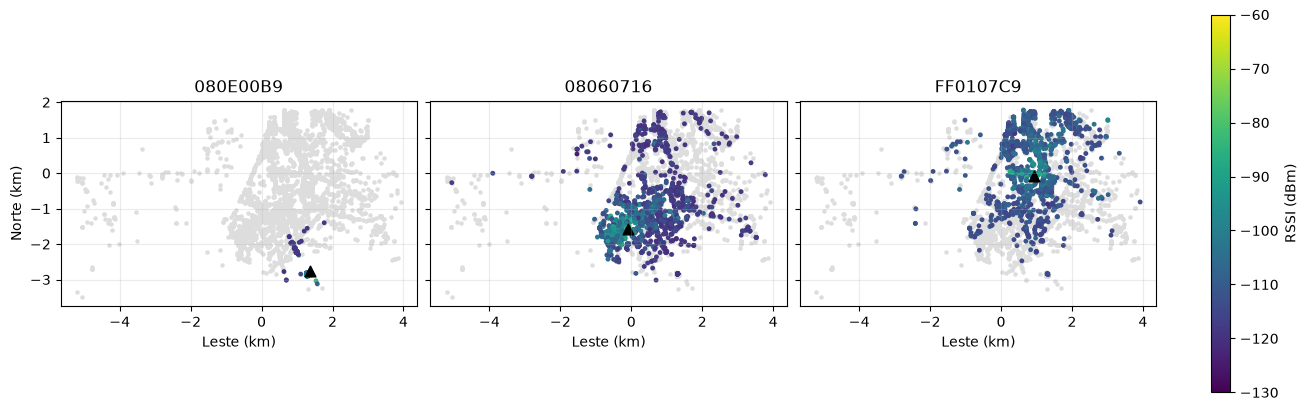
\includegraphics[width=.92\textwidth,height=.43\textheight,keepaspectratio]{figures/01_localizacao_03.png}
{\par\scriptsize RSSI por receptor; apenas dados de treino. Fonte: Antwerp, Aernouts et al.\par}
\begin{itemize}\footnotesize
\item Vários locais podem produzir sinais semelhantes: o problema é ambíguo.
\item Recepção ausente vira NaN; para os modelos, usamos um código fixo de \ensuremath{-}140.
\item A identidade dos gateways importa: não fazemos média dos RSSIs entre receptores.
\item Dias anteriores treinam; dias intermediários validam; dias posteriores testam.
\end{itemize}
\end{frame}

\begin{frame}{Erro para quem decide}{Voltar ao Colab \textperiodcentered{} passos 4 a 6}
\begin{itemize}\setlength{\itemsep}{.7em}
\item Erro de localização em metros: mediana e percentil 90.
\item Comparar baseline e modelo no mesmo teste.
\item Sálvora: concentração espacial pode favorecer uma estimativa quase constante.
\item Esse erro serviria para achar uma ferramenta numa sala? E um ativo numa região?
\end{itemize}
\end{frame}

\begin{frame}{Pausa técnica}{5 min \textperiodcentered{} estamos no minuto 70}
\begin{itemize}\setlength{\itemsep}{.7em}
\item Salve sua cópia do notebook.
\item Se ficou para trás, consulte as saídas salvas no notebook.
\item Próxima prática é independente: basta abrir outro notebook.
\end{itemize}
\end{frame}

\begin{frame}{Prática 2 \textperiodcentered{} Como estará o enlace?}{40 min \textperiodcentered{} Colab 02}
\begin{itemize}\setlength{\itemsep}{.7em}
\item Goldoni et al.: um nó, 1.059 horas contínuas selecionadas pela continuidade.
\item Após fechar a hora t, prever a média de RSSI de t+1.
\item Persistência repete o último valor. Ridge combina valores passados.
\item Abrir 02\_forecasting.ipynb \textperiodcentered{} passos 0 a 3.
\end{itemize}
\end{frame}

\begin{frame}{A linha temporal vira uma tabela}{Desenhe antes de executar}
\centering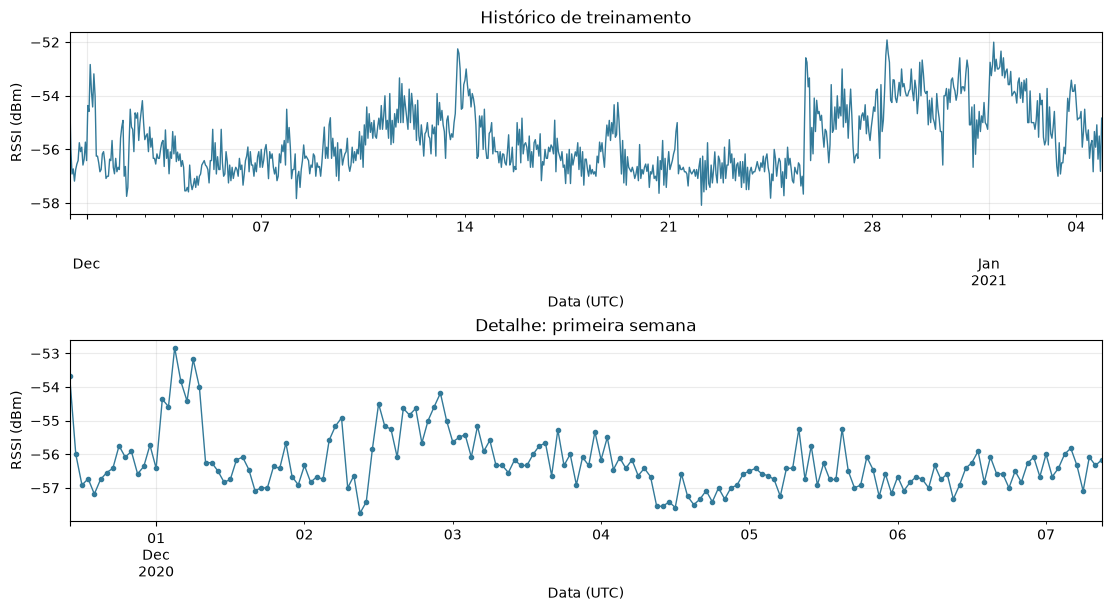
\includegraphics[width=.92\textwidth,height=.43\textheight,keepaspectratio]{figures/02_forecasting_01.png}
{\par\scriptsize Calendário e disponibilidade do histórico. Fonte: Goldoni et al.\par}
\begin{itemize}\footnotesize
\item Hora-alvo u=t+1: target=y(u); lag\_1=y(u\ensuremath{-}1); lag\_24=y(u\ensuremath{-}24).
\item Histórico: \ensuremath{-}80, \ensuremath{-}82, \ensuremath{-}81 dBm. Persistência para a próxima hora: \ensuremath{-}81 dBm.
\item Primeiros 80\% treinam; últimos 20\% testam.
\item Observações do teste entram no histórico só depois de chegarem. Uma hora à frente por vez.
\end{itemize}
\end{frame}

\begin{frame}{A previsão ajuda?}{Voltar ao Colab \textperiodcentered{} passos 4 a 7}
\begin{itemize}\setlength{\itemsep}{.7em}
\item RSSI em dBm; erro MAE/RMSE em dB.
\item MAE: erro absoluto médio. RMSE: maior peso para grandes erros.
\item O gráfico pode parecer excelente porque a série muda lentamente.
\item Se Ridge perder para persistência, temos uma conclusão útil. Não ajustar pelo teste.
\end{itemize}
\end{frame}

\begin{frame}{Clínica de armadilhas}{20 min \textperiodcentered{} quatro casos para votação}
\begin{itemize}\setlength{\itemsep}{.7em}
\item A. Localizar após recepção usando SNR do pacote.
\item B. Prever amanhã usando chuva medida amanhã.
\item C. Normalizar usando média de treino e teste juntos.
\item D. Usar o RSSI que chegou às 10 h para prever às 11 h.
\end{itemize}
\end{frame}

\begin{frame}{O instante resolve os casos}{Discuta o motivo, não só a resposta}
\begin{itemize}\setlength{\itemsep}{.7em}
\item A é válido: faz parte do fingerprint já recebido.
\item B vaza futuro; uma previsão meteorológica disponível antes seria outra entrada.
\item C contamina a transformação; ajuste somente no treino.
\item D é válido em forecasting sequencial de um passo.
\end{itemize}
\end{frame}

\begin{frame}{Split e overfitting}{A pergunta de generalização importa}
\begin{itemize}\setlength{\itemsep}{.7em}
\item Linhas próximas podem representar quase o mesmo local ou instante.
\item Nosso teste temporal não prova localização em áreas inéditas: isso exige avaliação espacial.
\item Excelente treino e teste ruim sugerem overfitting ou mudança de distribuição.
\item Escolher parâmetros repetidamente pelo teste faz o teste virar parte do treinamento.
\end{itemize}
\end{frame}

\begin{frame}{Uma boa métrica não fecha a decisão}{Conecte o erro ao uso}
\begin{itemize}\setlength{\itemsep}{.7em}
\item Mediana pode esconder a cauda: por isso olhamos P90 na localização.
\item MAE pequeno não garante detectar quedas raras do enlace.
\item RSSI das recepções não é taxa de entrega; faltam as transmissões não recebidas.
\item Validação em outra campanha e custo dos erros seriam próximos passos.
\end{itemize}
\end{frame}

\begin{frame}{Transfira a metodologia}{15 min \textperiodcentered{} síntese}
\begin{itemize}\setlength{\itemsep}{.7em}
\item LoRa fingerprint \(\rightarrow\) localização com pontos de acesso Wi-Fi.
\item RSSI horário \(\rightarrow\) throughput ou latência ao longo do tempo.
\item Antes de trocar o algoritmo, redefina unidade, target, instante e split.
\item Modelos mais complexos exigem uma razão operacional e dados adequados.
\end{itemize}
\end{frame}

\begin{frame}{Sua resposta de saída}{2 minutos \textperiodcentered{} individual ou em dupla}
\begin{itemize}\setlength{\itemsep}{.7em}
\item Escolha uma telemetria e escreva: quero prever \_\_\_\_ no instante \_\_\_\_.
\item Já conheço \_\_\_\_; reservarei \_\_\_\_ para teste.
\item Meu baseline será \_\_\_\_; o erro será medido em \_\_\_\_.
\item Antes de usar na rede, preciso verificar \_\_\_\_.
\end{itemize}
\end{frame}

\begin{frame}{Materiais e perguntas}{Continuar a partir de dois exemplos completos}
\begin{itemize}\setlength{\itemsep}{.7em}
\item Dois notebooks com aulas completas, comentários expansíveis, dados documentados e saídas salvas.
\item Fontes: Aernouts et al., Data 2018, doi:10.3390/data3020013; Goldoni et al., Computer Networks 2022, doi:10.1016/j.comnet.2021.108627.
\item Apoio: scikit-learn — Common pitfalls; Hyndman e Athanasopoulos — Forecasting: Principles and Practice.
\item Perguntas: qual seria sua primeira aplicação com dados da sua rede?
\end{itemize}
\end{frame}
\end{document}
